\ylDisplay{Laser ja lääts} % Ülesande nimi
{Tundmatu autor} % Autor
{lõppvoor} % Voor
{2015} % Aasta
{P 8} % Ülesande nr.
{3} % Raskustase
{
% Teema: Valgusõpetus
\ifStatement
Laser asub läätsest $2,5$ $f$ kaugusel ning optilisest peateljest kaugusel $f$, kus $f$ on läätse fookuskaugus. Laser on $45$$^{\circ}$ nurga all optilise peatelje suhtes. Teiselpool läätse olevale ekraanile tekib valgustäpp $0,5f$ võrra allpool optilist peatelge. Laserit liigutatakse paralleelselt peateljega $2f$ võrra läätse poole (laseri nurk ei muutu). Samal ajal liigutatakse ka ekraani paralleelselt optilise peateljega. Selle tulemusena asub valgustäpp ekraanil sama koha peal, kus alguses. Millise kauguse võrra nihutati ekraani? Kas oli võimalik, et ekraani ja laseri liigutamise ajal asus valgustäpp kogu aeg samas ekraani punktis?
\begin{center}
	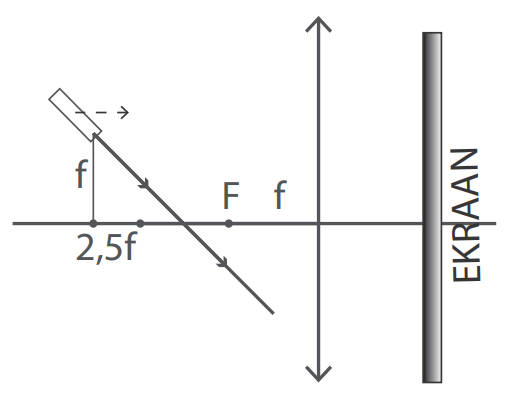
\includegraphics[width=0.5\linewidth]{2015-v3p-08-yl.PNG}
\end{center}
\fi
\ifHint
Ülesande lahendamisel tuleb kasutada kolmnurkade sarnasuse reegleid.
\fi
\ifSolution
\begin{center}
	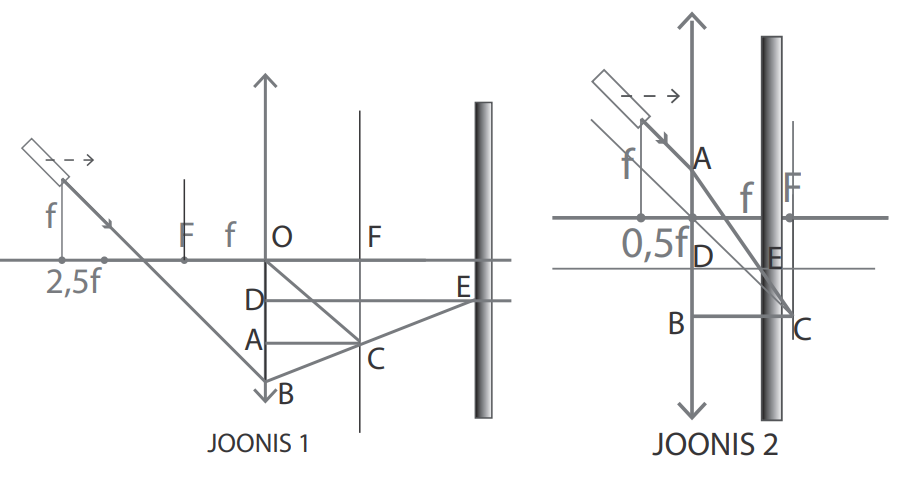
\includegraphics[width=0.5\linewidth]{2015-v3p-08-lah.PNG}
\end{center}
Leiame ekraani kauguse läätsest alguses. Sarnastest kolmnurkadest $4ABC$ ja $4DBE$ saame leida ekraani kauguse läätsest (lõik $DE$). Lõigu $DB$ pikkus on $f$, kuna $OB$ on $1,5f$ ning $OD$ on $0,5f$. 
Lõigu $AB$ pikkus on $0,5f$, kuna $OA$ $=$ $f$. Seega
\begin{center}
$\frac{DE}{DB} = \frac{AC}{AB}$ 
$\Rightarrow$
$\frac{DE}{f} = \frac{f}{0.5f}$
$\Rightarrow$
$DE = 2f$
\end{center}
Leiame ekraani kauguse läätsest pärast laseri nihutamist (vt. joonis 2). Sarnastest kolmnurkadest $4ABC$ ja $4ADE$ saame leida ekraani kauguse läätsest (lõik $DE$).
\begin{center}
$\frac{DE}{DA} = \frac{BC}{BA}$ $\Rightarrow$ $\frac{DE}{f} = \frac{f}{1,5f}$ $\Rightarrow$ $DE = \frac{2}{3}f$
\end{center}
Seega pidi ekraani nihutama läätsele lähemale $2f - \frac{2}{3} f$ $=$ $1 \frac{1}{3}f$. Valgustäppi ei ole võimalik kogu ekraani liigutamise ajal hoida samas punktis, sest kui laserkiir läbib fookust, siis peale läätse läbimist on kiir paralleelne optilise peateljega ning asub optilisest peateljest kaugusel $f$.
\fi
}